\section{Solución Propuesta}

\subsection{Arquitectura del Sistema}

\begin{figure}[t]
\centering
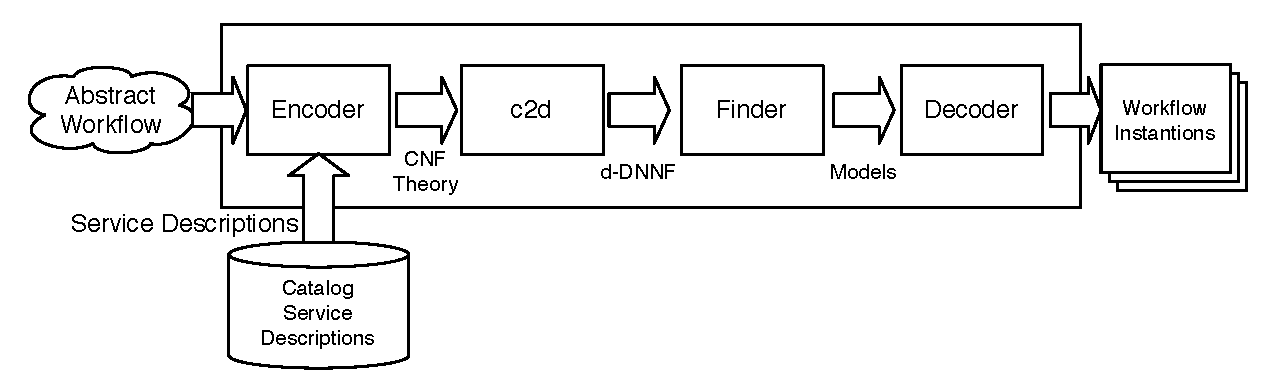
\includegraphics[width=.9\textwidth]{graphics/architecture}
\caption{Arquitectura del Sistema}
\label{fig:architecture}
\end{figure}

Se propone una arquitectura comprendida por un catálogo de descripciones de
servicio, el Codificador, el compilador c2d, el Buscador de mejores modelos, y
el Decodificador. La figura~\ref{fig:architecture} muestra la arquitectura global del sistema.
En esta infraestructura, una instancia del problema de instanciación de flujos
de trabajo se define como un flujo abstracto representado por una consulta
conjuntiva sobre servicios abstractos que es dada como entrada junto con un
conjunto de servicios concretos definidos por vistas de servicios abstractos.

El catálogo se carga con descripciones de servicios abstractos y concretos; cada
servicio es descrito en términos de atributos de entrada y salida y anotado con
un valor real que representa la utilidad QoS del servicio. La descripción de los
servicios concretos, que son definidos como vistas de los servicios abstractos,
puede ser generada de manera semiautomática o automática usando herramientas
tales como el sistema DEIMOS \cite{AmbiteISWC09}.

Una instancia de entrada de WIP es codificada como una teoría CNF cuyos modelos
corresponden a las intanciaciones del flujo de trabajo por el Codificador. El
compilador c2d, un componente \emph{off-the-shelf}, compila la fórmula CNF a
d-DNNF. El Codificador traduce las instancias WIP en teorías CNF que luego son
convertidas en d-DNNF usando c2d. El Buscador computa un mejor modelo dados los
parámetros QoS en tiempo lineal en el tamaño del d-DNNF resultante. Es
importante remarcar que el proceso de compilación necesita ser realizado sólo
una vez ya que no depende del valor de los parámetros QoS. Así, incluso si la
compilación resulta ser costosa en términos de tiempo, este costo puede ser
amortizado dado que el d-DNNF resultante puede ser usado para conseguir mejores
instanciaciones con respecto a múltiples valores de los parámetros QoS.
Finalmente, el Decodificador traduce el mejor modelo retornado por el Buscador
a una instanciación de flujo de trabajo que resuelve el WIP.

Dado un CNF que codifica un WIP, su d-DNNF es una representación compacta de
todas las instanciaciones del flujo de trabajo. Es decir, uno puede generar de
una manera libre de \emph{backtracking} todas las instanciaciones del flujo de
trabajo. Si el usuario está interesado en una mejor instanciación dados
parámetros de QoS, entonces esta se puede computar en tiempo lineal en el tamaño
del d-DNNF. Si el usuario está interesado en todas las mejores instanciaciones,
estas pueden ser computadas en tiempo lineal en su número. Finalmente, si el
usuario está interesado en todas las instanciaciones, estas también pueden ser
computadas en tiempo lineal en su número. En los últimos dos casos, si ese
número es exponencial (en el tamaño de la entrada), la enumeración de las
instanciaciones también lo es pero esta complejidad es intrínsica al problema y
por lo tanto no puede ser evitada.

\subsection{Teorías Lógicas}

Se usa una solución similar a la descrita en
\cite{arvelo:aaai06} para codificar el WIP. 
Se identifican instanciaciones del flujo de trabajo enumerando los modelos de
una teoría lógica
$\Delta=\Delta_{com}\cup\Delta_{id}^1\cup\cdots\Delta_{id}^N$
donde $\Delta_{com}$ especifica cómo combinar $N$ copias independientes de la teoría
$\Delta_{id}$ que cubren los objetivos en $W$.
Cada $\Delta^i_{id}$ es una copia etiquetada $\Delta_{id}$ en la cual cada
literal 
$\ell$ está etiquetado como $\ell^i$.
La teoría \emph{Instantiation Description} (ID) $\Delta_{id}$ consiste de
diferentes grupos de cláusulas que garantizan que sus modelos están en
correspondencia con instanciaciones parciales, mientras que la teoría
$\Delta_{com}$ contiene cláusulas adicionales para garantizar una combinación
correcta y completa de instanciaciones parciales para una instanciación
completa.
La teoría ID $\Delta_{id}$ consiste de las siguientes variables:

\begin{enumerate}[--]
\item $\{v_0,\ldots,v_n\}$ para indicar qué $V_i$ se usa, o $v_0$ para indicar el ID nulo.
\item $\{g_1,\ldots,g_m\}$ para indicar objetivos cubiertos por la vista.
\item $\{z_{j,k,i}\}$ para indicar que el objetivo $j$ en $W$ está cubierto por el objetivo $k$ en $V_i$.
\item $\{t_{x,y}\}$ para indicar que la variable/constante $x$ en $W$ está asociada a la variable/constante $y$ en la vista.
\end{enumerate}

Los rangos de los índices para las variables $z$ y $t$ dependen del problema.

Las siguientes cláusulas codifican el problema WIP en términos de los WIDs.
Rajaraman et al.\ \cite{RajaramanSU95} mostraron que para consultas sin negación
o comparaciones aritméticas, pero con constantes, y $m$ objetivos y $k$
variables en la cabeza del flujo de trabajo, es suficiente considerar
instanciaciones de longitud a lo más $N=m+k$.

\begin{enumerate}[C10.]
\item[C1.] (Al menos una vista es usada): $\bigvee_{i=0}^n v_i$.
\item[C2.] (A lo más una vista es usada): $\neg v_i\lor\neg v_j$ para $i\neq j$.
\item[C3.] (Vista nula implica nulidad): $v_0 \Rightarrow \neg g_j$ para $1\leq j\leq m$.
\item[C4.] (Las vistas son útiles): $v_i \Rightarrow \bigvee_{j=1}^m g_j$ para $1\leq i\leq n$.
\item[C5.] (Objetivos cubiertos máximo una vez): $z_{j,k,i} \Rightarrow \neg z_{j,l,i}$ para $i,j,k,l$ apropiados.
\item[C6.] (Alcance de las vistas): $v_i \Rightarrow \neg g_j$ para objetivos que no pueden ser cubiertos por $V_i$.
\item[C7.] (Consistencia): $v_i \land g_j \Leftrightarrow \bigvee z_{j,k,i}$ para $i,j,k$ apropiados.
\item[C8.] (Variables muertas): $v_i \Rightarrow \neg t_{x,y}$ para todo $x,y$ con $y\notin V_i$.
\item[C9.] (1-1 para $\exists$ vars): $v_i \land t_{x,y} \Rightarrow \neg t_{x,y'}$ para todas las variables existenciales $y,y'\in V_i$.
\item[C10.] (Distinguidos): $v_i \Rightarrow \neg t_{x,y}$ para $x$ distinguido y $y\in V_i$ existencial .
\item[C11.] (Existencial): $v_i\land t_{x,y}\Rightarrow g_j$ para exist.\ $y\in V_i$ y objetivos $g_j$ que contengan $x$.
\item[C12.] (Coincidencia): $v_i\land z_{j,k,i} \Rightarrow t_{x,y}$ para todo
$x,y$ que deban coincidir si $g_j$ es cubierto por el objetivo $k$ en $V_i$.
\item[C13.] (Si todas las variables en $V_i$ son distinguidas, sólo cubre un objetivo): $v_i \land g_j \Rightarrow \neg g_k$ para vistas $v_i$ apropiadas.
\end{enumerate}

Estas son las mismas cláusulas usadas por \mcdsat\ para codificar QRPs \cite{arvelo:aaai06}.
Para poder manejar símbolos constantes apropiadamente, las cláusulas deben ser
mejoradas con:

\begin{enumerate}[C10.]
\item[C14.] (Inconsistencia directa 1): $t_{x,A} \Rightarrow \neg t_{x,B}$.
\item[C15.] (Inconsistencia directa 2): $t_{A,x} \Rightarrow \neg t_{B,x}$.
\item[C16.] (Inconsistencia directa 3): $\neg t_{A,B}$.
\item[C17.] (Transitividad 1): $v_i\land t_{A,y}\land t_{x,y}\land t_{x,z}\Rightarrow t_{A,z}$.
\item[C18.] (Transitividad 2): $v_i\land t_{y,A}\land t_{y,x}\land t_{z,x}\Rightarrow t_{z,A}$.
\end{enumerate}

El problema principal al manejar constantes es estar seguro de que no haya dos
constantes distintas asociadas entre sí directa o indirectamente. Las cláusulas
C14--C16 quitan asociaciones directamente inconsistentes, mientras que las
últimas dos cláusulas implementan propagación de asociaciones restringida que
quita inconsistencias indirectas.
De la misma manera, la teoría $\Delta_{com}$ que especifica instanciaciones
completas contiene las siguientes cláusulas:

\begin{enumerate}[C10.]
\item[C19.] (Cubrir todos los objetivos): $\bigvee_{j=1}^m g^i_j$ para $1\leq i\leq N$.
\item[C20.] (Cobertura disjuntiva): $g^i_k \Rightarrow \neg g^j_k$ para $i\neq j$.
\item[C21.] (Quitar simetrías): $g^i_j \Rightarrow \bigvee_{k=1}^{j-1} g^{i-1}_k$
            para $1\leq j\leq m$ y $1\leq i\leq N$.
\item[C22.] (Inconsistencia directa 4): $t^i_{x,A} \Rightarrow \neg t^j_{x,B}$.
\end{enumerate}

Estas cláusulas proveen una caracterización correcta y completa de WIPs en el
sentido en que sus modelos están en correspondencia con las instanciaciones del
flujo de trabajo.

\subsection{Parámetros QoS}

Para los parámetros QoS, se supone un modelo de agregación aditiva simple en el
que cada vista
$V_i$ está asociada con un costo $c(V_i)$ (negativo si tratamos de utilidad),
y una instanciación completa con la suma de los costos de sus vistas.
Una instanciación óptima o mejor es una con costo mínimo, y el valor óptimo del
WIP es el costo de una instanciación óptima.
Un WIP siempre tiene un valor óptimo bien definido (si no hay instanciaciones,
su costo es $\infty$), pero puede tener múltiples mejores instanciaciones.
El WIP con costos consiste en encontrar todas las instanciaciones óptimas o una
instanciación, esto depende de la aplicación particular.
En la formulación propuesta, esto puede hacerse a partir del d-DNNF que codifica
$\Delta$
usando la función de calidad de literales $r$ que asigna
$r(\ell)=c(V_i)$ si
$\ell=v_i$, y $r(\ell)=0$ if $\ell\notin\{v_1,\ldots,v_n\}$.
